\makeatletter
\def\input@path{{../../}}
\makeatother
\documentclass[../../main.tex]{subfiles}

\graphicspath{
	{../../img/}
	{../img/}
	{img/}
}

\begin{document}
\section{Интеграл Эйлера-Пуассона}
	\begin{defn}
		\emph{Интегралом Эйлера-Пуассона} называется несобственный интеграл 
		\begin{equation}
		 	\label{lec17:1}
            \int\limits_0^{+\infty}e^{-x^2}dx = \lim\limits_{A\to +\infty} 
            I(A),
		\end{equation}
        где
		\begin{equation}
		 	\label{lec17:2}
            \begin{cases}
                I(A) = \int\limits_0^{A}e^{-x^2}dx, \\
                A \geq 0.
            \end{cases}
		\end{equation}
        \end{defn}
		
		\begin{theorem}
		 (О вычислении интеграла Эйлера-Пуассона)
		 \begin{equation}
          \label{lec17:3}
		  \int\limits_0^{+\infty}e^{-x^2}dx = \frac{\sqrt{\pi}}{2}.
		 \end{equation}

		\end{theorem}
		
\begin{proof}
	Для $\fix A > 0$ рассмотрим 2И
	\begin{equation}
		\label{lec17:4}
		F(A) = \iint\limits_De^{-(x^2 + y^2)}dxdy,
	\end{equation}
	где
	\begin{equation}
        \label{lec17:5}
		D :
		\begin{cases}
			0 \leq x \leq A,\\
			0 \leq y \leq A\\
		\end{cases}
		\text{--- квадрат в $\R^{2}$.}
	\end{equation}
	\begin{center}
      \begin{minipage}{.5\textwidth}
		\centering
		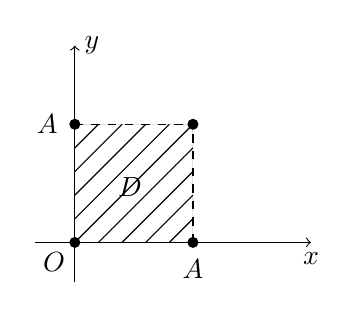
\begin{tikzpicture}
            \coordinate (left) at (-0.5, 0.0);
            \coordinate (right) at (3.0, 0.0);
            \coordinate (top) at (0.0, 2.5);
			\coordinate (bottom) at (0.0, -0.5);
            \coordinate (center) at (0.0, 0.0);
            
            \draw[->] (left) -- (right);
            \draw[->] (bottom) -- (top);
            
            \draw[-] (0, 0) -- (1.5, 1.5);
            \draw[-] (0, 0.3) -- (1.2, 1.5);
            \draw[-] (0, 0.6) -- (0.9, 1.5);
            \draw[-] (0, 0.9) -- (0.6, 1.5);
            \draw[-] (0, 1.2) -- (0.3, 1.5);
            
            \draw[-] (0.3, 0) -- (1.5, 1.2);
            \draw[-] (0.6, 0) -- (1.5, 0.9);
            \draw[-] (0.9, 0) -- (1.5, 0.6);
            \draw[-] (1.2, 0) -- (1.5, 0.3);

            \draw (center) node[anchor=north east] {$O$};
            \draw (right) node[anchor=north] {$x$};
            \draw (top) node[anchor=west] {$y$};

            \draw[fill=black, dashed] (0, 1.5) -- (1.5, 1.5);
            \draw[fill=black, dashed] (1.5, 0) -- (1.5, 1.5);
				
            \draw (0.7,0.7) node[anchor=center] {$D$};
				
            \draw (1.5, -0.1) node[anchor=north] {$A$};
            \draw (-0.35,1.5) node[anchor=center] {$A$};
            
            \fill [black] (1.5,1.5) circle (2pt);
            \fill [black] (1.5,0) circle (2pt);
            \fill [black] (0, 1.5) circle (2pt);
            \fill [black] (0, 0) circle (2pt);
            
			\end{tikzpicture}
		\end{minipage}
	\end{center}
	
    Пусть $D_1 \subset D \subset D_2$. 
 
    \begin{center}
      \begin{minipage}{.5\textwidth}
        \centering
			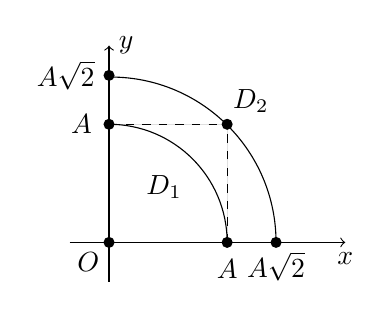
\begin{tikzpicture}
				\coordinate (left) at (-0.5, 0.0);
				\coordinate (right) at (3.0, 0.0);
				\coordinate (top) at (0.0, 2.5);
				\coordinate (bottom) at (0.0, -0.5);
				\coordinate (center) at (0.0, 0.0);
				
				\draw[->] (left) -- (right);
				\draw[->] (bottom) -- (top);
				
				\draw (center) node[anchor=north east] {$O$};
				\draw (right) node[anchor=north] {$x$};
				\draw (top) node[anchor=west] {$y$};
				
				\draw (2.121, 0) arc(0:90:2.1);
				\draw (1.5, 0) arc(0:90:1.5);
				
				\draw[fill=black, dashed] (0, 1.5) -- (1.5, 1.5);
				\draw[fill=black, dashed] (1.5, 0) -- (1.5, 1.5);
				
				\draw (0.7,0.7) node[anchor=center] {$D_1$};
				\draw (1.8,1.8) node[anchor=center] {$D_2$};
				
				\draw (2.121, 0) node[anchor=north] {$A\sqrt{2}$};
				\draw (1.5, -0.1) node[anchor=north] {$A$};
                \draw (-0.55,2.121) node[anchor=center] {$A\sqrt{2}$};
                \draw (-0.35,1.5) node[anchor=center] {$A$};
				
				\fill [black] (1.5,1.5) circle (2pt);
				\fill [black] (1.5,0) circle (2pt);
				\fill [black] (0, 1.5) circle (2pt);
				\fill [black] (0, 0) circle (2pt);
				
				\fill [black] (0,2.121) circle (2pt);
				\fill [black] (2.121,0) circle (2pt);
			\end{tikzpicture}
		\end{minipage}
     \end{center}
 
     \begin{equation}
		 	\label{lec17:6}
            \begin{cases}
                D_1 : x^2 + y^2 = A^2,\\
                D_2 : x^2 + y^2 = 2A^2,\\
                x \geq 0,\ y \geq 0.\\
            \end{cases}
		\end{equation}
  Тогда, используя неотрицательность подынтегральной 
  функции в \eqref{lec17:4}, а также аддитивность и монотонность ОИ, имеем:
	\begin{equation}
		\label{lec17:7}
		\iint\limits_{D_1}e^{-(x^2 + y^2)}dxdy \leq F(A) \leq
		\iint\limits_{D_2}e^{-(x^2 + y^2)}dxdy.
	\end{equation}
    Для $\fix R > 0$, используя полярную замену, вычислим:
	\begin{equation}
        \label{lec17:8}
		G(R) = \iint\limits_{\substack{
		x^2 + y^2 \leq R^2 \\
		x \geq 0 \\
		y \geq 0
		}}e^{-(x^2 + y^2)}dxdy.
	\end{equation}
	Имеем:
    \begin{equation*}
        G(R) =
        \left[
		\left\{
        \begin{gathered} 
        x = r \cos \phi,\\
        y = r \sin \phi,\\
        |I| = r.
        \end{gathered}
        \right. \quad
        \begin{gathered}
        r\vert_0^R\\
		\phi \vert_0^{\frac{\pi}{2}}\\
        \end{gathered}
        \right]
        = \iint\limits_{\substack{0\leq\phi\leq \frac{\pi}{2}\\
				0 \leq r \leq R}}r e^{-r^2}drd\phi =
        \left[ \phi \right]_0^{\frac{\pi}{2}} \cdot
        \left[ -\frac{e^{-r^2}}{2} \right]_0^{R} =
        \frac{\pi}{4}(1 - e^{-R^2}).
	\end{equation*}
	Отсюда для $R = A$ и $R = A\sqrt{2}$ в силу \eqref{lec17:7} получаем:
	\begin{equation}
	 \frac{\pi}{4}(1 - e^{-A^2}) \leq F(A) \leq
	 \frac{\pi}{4}(1 - e^{-2A^2})
	\end{equation}
    Следовательно, при $A \to +\infty$ получаем:
    \begin{equation}
    \exists F(+\infty)=\lim\limits_{A\to+\infty}F(A) = \frac{\pi}{4}.
    \end{equation}
    С другой стороны, вычисляя \eqref{lec17:4} через повторные, имеем:
    \begin{equation*}
     F(A)= \int\limits_0^{A}dx\int\limits_0^{A}e^{-(x^2+y^2)}dy = 
     \int\limits_0^{A}e^{-x^2}dx \int\limits_0^{A}e^{-y^2}dy = I^2(A).
    \end{equation*}
    Таким образом, $I^2(A) =
    F(A) \xrightarrow[A\to +\infty]{} \dfrac{\pi}{4}$.
    
    Учитывая, что в \eqref{lec17:1}, \eqref{lec17:2} 
    подынтегральная функция неотрицательна, т.~е.
    $I(A) \geq 0$, получаем:
    \[
     I(A)\xrightarrow[A\to +\infty]{} 
     \sqrt{\frac{\pi}{4}} = \frac{\sqrt{\pi}}{2},
	\]
	что соответствует \eqref{lec17:3}.
\end{proof}

\begin{crl*}
 (Обобщение интеграла Эйлера-Пуассона)
    \begin{equation}
		 	\label{lec17:9}
		 	\forall a \geq 0 \implies \int\limits_0^{+\infty}e^{-ax^2}dx = 
		 	\frac{1}{2}\sqrt{\frac{\pi}{a}}
    \end{equation}
\end{crl*}
\begin{proof}
 Для доказательства достаточно воспользоваться заменой
 \begin{equation*}
  t = x\sqrt{a}\Big|_0^{+\infty} \implies x = \frac{t}{\sqrt{a}} 
  \implies dx = \frac{dt}{\sqrt{a}}.
 \end{equation*}
  Тогда
\begin{equation*}
    \int\limits_0^{+\infty}e^{-ax^2}dx = 
    \int\limits_{0}^{+\infty}\frac{e^{-t^2}dt}{\sqrt{a}} = 
    \frac{1}{\sqrt{a}} \int\limits_{0}^{+\infty}e^{-t^2}dt 
    \overset{\eqref{lec17:1}}=
    \frac{\sqrt{\pi}}{2\sqrt{a}} =
    \frac{1}{2}\sqrt{\frac{\pi}{a}}.
    \qedhere
\end{equation*}
\end{proof}
Отметим, что интеграл Эйлера-Пуассона играет 
важную роль в теории вероятностей.

\begin{examples}
~
 \begin{enumerate}
  \item Пусть  $A>0$ и $b, c \in \R$, тогда, выделяя полный квадрат, имеем:
  \begin{equation}
  \begin{gathered}
   \int\limits_{-\infty}^{+\infty}e^{-ax^2 + bx + c}dx =
   \int\limits_{-\infty}^{+\infty}e^{-a(x + \frac{b}{a})^2 +
   \frac{b^2}{4a} - c}dx =
   \left[t = x + \left.\frac{b}{2a}\right|_{-\infty}^{+\infty} \right] = \\
   = e^{\frac{b^2-4ac}{4a}} \int\limits_{-\infty}^{+\infty}e^{-at^2}dt =
   2e^{\frac{b^2-4ac}{4a}} \int\limits_0^{+\infty}e^{-at^2}dt=
   \sqrt{\frac{\pi}{a}}e^{\frac{b^2-4ac}{4a}}.
  \end{gathered}
  \label{lec17-exmp1}
  \end{equation}

  \item Для $a>0$ и $b \in \R$ рассмотрим и вычислим интеграл:
  \begin{gather*}
    \int\limits_{-\infty}^{+\infty}e^{-ax^2}\ch{bx}\:dx =
    \left[\ch{bx} = \frac{e^{bx} + e^{-bx}}{2} \right] =
	\\
    =\frac{1}{2}\left(\int\limits_{-\infty}^{+\infty}e^{-(ax^2 - bx)}dx  +
    \int\limits_{-\infty}^{+\infty}e^{-(ax^2 + bx)}dx\right)
    \stk{lec17-exmp1}{=} \frac{1}{2}\cdot\sqrt{\frac\pi a}
    \left(e^{\frac{(-b)^2}{4a}} + e^{\frac{b^2}{4a}}\right) =
    \sqrt{\frac{\pi}{a}}\cdot e^{\frac{b^2}{4a}}.
  \end{gather*}
  \item Для $n \in N_0$ рассмотрим интеграл 
  \[I_n = \int\limits_{0}^{+\infty} e^{-x^2}x^{2n}dx.\]
  
  Имеем:
  \[
   I_0 = \int\limits_0^{+\infty}e^{-x^2}dx = \frac{\sqrt{\pi}}{2}.
  \]
  
  Для $\forall n \in \N$, интегрируя по частям, получаем:
  \begin{gather*}
  I_n = -\frac{1}{2} \int\limits_{0}^{+\infty}x^{2n-1}d{(e^{-x^2})}
  = -\frac{1}{2}\left(\left[x^{2n-1}e^{-x^2}\right]_0^{+\infty} - 
  \int\limits_{0}^{+\infty}e^{-x^2}d{(x^{2n-1})}\right) =
  \\
    =\left[ x^{2n-1}e^{-x^2}\Big|_0^{+\infty}  =
    \lim\limits_{A\to +\infty} \frac{x^{2n -1}}{e^{x^2}}
    \overset{\lopital}{=} \dots = 0
    \right] =
    \frac{2n-1}{2}\int\limits_{0}^{+\infty}e^{-x^2}x^{2n-2}dx =
    \frac{2n-1}{2}I_{n-1}.
  \end{gather*}
  т.~е. 
  \[\begin{cases}
     I_n = \frac{2n-1}{2}I_{n-1},\ n \in \N,\\
     I_0 = \frac{\sqrt{\pi}}{2}.
    \end{cases}\]
  Отсюда последовательно получаем 
  \begin{gather*}
  I_n = \frac{2n-1}{2} \cdot \frac{2n-3}{2} \cdot I_{n-2}= \dots =
    \frac{2n-1}{2} \cdot \frac{2n-3}{2} \cdot \dots
    \cdot \frac{3}{2} \cdot \frac{1}{2} \cdot I_0 =
  \\
    =\frac{1\cdot 3 \cdot 5 \cdot \dots \cdot (2n-1)}{2^{n}}\cdot
    \frac{\sqrt{\pi}}{2} = 
    \frac{(2n-1)!!}{2^{n+1}}\sqrt{\pi}.
  \end{gather*}
  \item Для $a \in \R$ вычислим  \[I(a) = 
  \int\limits_{0}^{+\infty}e^{-\left(x^2+\frac{a^2}{x^2}\right)}dx.\]
  Выделяя полный квадрат, получаем:
  \begin{gather*}
   I(a) = 
   \left[
    \begin{array}{ccc}
      x^2 + \frac{a^2}{x^2} = (x - \frac{|a|}{x})^2 + 2|a|,\\
      t = 
      \left. x - \frac{|a|}{x} \right|_{-\infty}^{+ \infty},\\
      x^2 - tx - |a| = 0 \iff \\ \iff
      x = \frac{t \pm \sqrt{t^2 + 4|a|}}{2} 
      \xrightarrow[t \to \mp \infty]{} \mp \infty \implies \\
      \implies x = \frac{t - \sqrt{t^2 + 4|a|}}{2}, \\
      dx = d(\frac{t - \sqrt{t^2 +4|a|}}{2}) =
      \frac{1}{2}\big(1 - \frac{t}{\sqrt{t^2 + 4|a|}}\big)dt.
     \end{array}
    \right]
    =\frac{1}{2}e^{2|a|}
    \int\limits_{-\infty}^{+\infty}e^{-t^2}
    \left(1 - \frac{t}{\sqrt{t^2 + 4|a|}}\right) dt = 
    \\
    =\frac{1}{2}e^{2|a|}\left(
    \underbrace{\int\limits_{-\infty}^{+\infty}e^{-t^2}dt}_{\text{чётная}} 
    \:-\:
    \underbrace{\int\limits_{-\infty}^{+\infty}
    \frac{te^{-t^2}}{\sqrt{t^2 + 4|a|}}dt}_\text{нечётная}\right) =
    e^{2|a|}\int\limits_{0}^{+\infty}e^{-t^2}dt 
    \overset{\eqref{lec17:1}}{=} \frac{\sqrt{\pi}}{2}e^{2|a|}.
  \end{gather*}
 \end{enumerate}
\end{examples}
\end{document}
